% Springer Nature LaTeX template, version 3.1 (December 2024)
\documentclass[pdflatex,sn-mathphys-num]{sn-jnl}

\usepackage[T1]{fontenc}
\usepackage[utf8]{inputenc}
\usepackage{graphicx}
\usepackage{amsmath}
\usepackage{amssymb}
\usepackage{booktabs}
\usepackage{algorithm}
\usepackage{algorithmicx}
\usepackage{algpseudocode}
\usepackage{listings}
\usepackage{multirow}
\usepackage{xcolor}
\usepackage{array}
\usepackage{tabularx}

\graphicspath{{./}}
\raggedbottom

\begin{document}

\title[TRACE]{TRACE: Structural Planning, Tool-Grounded Multi-Agent Verification, and Traceability-Guided Local Repair for LLM-Based Java Unit Testing}

% Author and affiliation placeholders: replace before submission.
\author*[1]{\fnm{First} \sur{Author}}\email{author@example.com}
\affil*[1]{\orgdiv{Department}, \orgname{Institution}, \orgaddress{\city{City}, \country{Country}}}

\abstract{Java unit test generation using large language models (LLMs) still faces limitations in structural planning, controlling the scope of bug fixes, and the reliability of verification decisions. This research proposes TRACE with three contributions: (1) Structural Planning based on AST/CFG to construct atomic scenarios with structural objectives and auditable evidence sources; (2) Traceability-Guided Scenario-Local Repair (TGSLR), maintaining a bidirectional mapping of scenario--test to limit the scope of fixes and perform regression checks before acceptance; (3) Tool-Grounded Specialized Multi-Agent Verification, combining specialized verification roles to detect incorrect acceptances, trace the root cause, and route bug fixes. The three contributions are independently evaluated using three separate datasets. RQ1 uses 150 focal methods from SF110, generating 600 runs with two LLM configurations. PLANNED raised the aggregate execution rate from 58.00\% to 88.33\% and the end-to-end branch coverage from 43.51\% to 70.58\%, with a token volume of about 2.03 times DIRECT. Improvements in execution and three structural quality indicators were significant after the Holm correction by each model; the benefit on co-successful execution pairs was more pronounced in Gemini and unstable in DeepSeek. RQ2 used 100 error units from LIBRO--Defects4J. TGSLR achieved a 60\% success rate of fixes, compared to 46\% of local fixes without scenario context and 76\% of full-class regeneration. The advantage over the local fix method was not significant after Holm; on successful fixes, TGSLR changed by an average of 10.48 lines less than full-class regeneration, but this is only a descriptive comparison. RQ3 uses its own verification dataset of 73 cases from 14 Java projects. With Gemini, specialized verification reduces the false-acceptance rate from 57.69\% to 26.92\% and increases routing accuracy from 42.59\% to 66.67\%, at the cost of input tokens being 2.97 times that of a general reviewer. The RQ3 results are exploratory. Overall, the study clarifies the value and trade-offs of planning, traceable debugging, and specialized verification in LLM-based testing.}

\keywords{unit test generation; large language models; structural planning; traceability-guided repair; multi-agent verification; mutation testing; Java}

\maketitle

\nocite{bib1,bib2,bib3,bib4,bib5,bib6,bib7,bib8,bib9,bib10,bib11,bib12,bib13,bib14,bib15,bib16,bib17,bib18,bib19,bib20,bib21,bib22,bib23,bib24,bib25}

\section{Introduction}\label{sec:introduction}

\subsection{The Importance of Unit Testing}\label{subsec:importance}

Software testing is an essential but labor-intensive activity in the software development lifecycle because it directly affects the quality, reliability, and maintainability of the system. Among these, unit testing provides the first line of verification by checking small program units such as classes and methods. Detecting errors at this level helps shorten the process of pinpointing causes, limits errors from spreading to integration and deployment stages, and supports refactoring and regression detection. However, manually building a high-quality unit test suite---including input data, edge cases, error paths, and appropriate assertions---still requires significant time and knowledge of both the source code and the project environment \cite{bib1,bib2,bib11}.

The development of large language models (LLMs) opens up the possibility of automating this activity. Thanks to their interpretation and code generation capabilities, LLMs can analyze the focal method, propose test scenarios, generate JUnit code, and construct assertions from the provided context. Recent studies show that LLMs can generate tests achieving significant coverage \cite{bib1,bib2,bib11}. Adaptive focal context along with dependency and build information at the project level helps increase the practical validity of the output \cite{bib3,bib5}, while industrial deployment emphasizes the role of pre-execution filters before accepting improved tests \cite{bib4}. However, a useful test suite not only needs to compile and run but also must achieve the intended structural objectives, detect faults, and maintain quality; therefore, line/branch coverage \cite{bib1,bib2,bib11}, mutation score \cite{bib12}, and test-smell evidence \cite{bib13} provide additional perspectives rather than mutually substitutive measures.

\subsection{Limitations of existing LLM-based methods}\label{subsec:limitations}

Existing methods still face a significant gap between generating test code and producing a usable test suite. LLMs may call non-existent APIs, choose incorrect imports or dependencies, violate type or access rules, or create fixtures and mocks incompatible with the class to be tested. Many tests thus fail to compile; tests that compile successfully can still fail at runtime due to incorrect initialization, unexpected exceptions, or assertions that do not match observed behavior. ChatTester, ChatUniTest, TestART, and TestLoter use responses During compilation, execution, or coverage in the generation--validation--repair cycles \cite{bib2,bib3,bib9,bib10}; CATGen emphasizes structured project context, deterministic scaffolding, and static post-processing \cite{bib5}; while large-scale studies show that results are still sensitive to prompt and context configuration \cite{bib11}. These advances do not automatically ensure that tests have correctly implemented the target scenario, have a reliable oracle, or have been fixed within a scope that does not break already verified tests.

Three specific gaps have not yet been satisfactorily addressed. First, standardized test design techniques such as equivalence partitioning, boundary-value analysis, and structural coverage provide auditable rules to infer test conditions \cite{bib6}, while TestAgent's Requirement Planner generates structured test requirements from semantic analysis of the method \cite{bib7}. Therefore, the individual impact of structural planning versus direct generation is unclear when keeping the LLM, context, number of test methods, and generation budget fixed. Second, ChatTester, ChatUniTest, TestART, and TestLoter use feedback to fix test failures \cite{bib2,bib3,bib9,bib10}, but do not publish an immutable bidirectional contract between the atomic scenario and the test method; therefore, the benefits of scenario-local repair in terms of cost, edit scope, repair iterations, and regression need to be measured directly against fixing a failing test method without scenario context and regenerating the entire class. Third, TestAgent has combined agent roles with tool APIs and allowed the Reviewer to handle execution, coverage, and mutation evidence, while MAGISTER separates the Analyzer, Test Generation, Executor, and Refiner Agent \cite{bib7,bib8}. The gap that TRACE aims at, therefore, is not the absence of tools in general, but the fact that verification has not yet been separated into specialized evidence streams, linked to an immutable scenario identity, and aggregated into a primary failure cause along with a repair route at the scenario level. The increased accuracy of this design needs to be distinguished from Basic Tool Gates and a General-Purpose Reviewer provided along with evidence.

\subsection{Overview of TRACE}\label{subsec:overview}

TRACE addresses these gaps through a seven-block pipeline. (1) Input and Repository Analysis receives a Java repository, focal class, and focal method, then extracts build metadata, dependencies, and AST/CFG into a repository context. (2) Structural Planning applies predicate-induced partitions, boundary values, branch outcomes, and exception paths to create an Immutable Atomic Scenario Plan consisting of S01, S02, \ldots{}, SN. (3) Traceable Scenario Test Generation maintains a bijective mapping $S_i$ \ensuremath{\leftrightarrow} $T_i$ between each scenario and exactly one test method. (4) Tool Execution uses Maven/Gradle and JUnit to produce build/run evidence, employs JaCoCo and PIT for coverage/mutation measurements linked to individually executed tests, and uses tsDetect to assess test smells at the test file or generated class level \cite{bib11,bib12,bib13}. (5) Specialized Multi-Agent Verification for the Conformance Agent, Compilation/Runtime Diagnosis Agent, and Coverage/Mutation Analysis Agent handles independent aspects once the corresponding evidence is ready, then the Evidence Aggregator merges the results according to the scenario ID. (6) Repair Routing distinguishes scenario-local defects, shared-infrastructure defects, and context-insufficient cases; local repair only changes test methods under ownership and must go through a regression check. (7) The Final Test Suite stores test code, scenario--test mapping, verification evidence, repair history, and unresolved/abstained cases.

\subsection{Main contributions}\label{subsec:contributions}

This study has three main contributions. First, Auditable Test-Design-Technique-Grounded Structural Planning: the study proposes a Structural Planner separated from the Generator, combining repository context with AST/CFG to infer predicate-induced partitions, boundary values, branch outcomes, and exception paths according to standardized test design techniques \cite{bib6}. The Planner releases an immutable atomic scenario plan in which each scenario has an ID, activation conditions, expected behavior with source evidence, and a specific structural target at the line, branch/predicate outcome, or exception path level. Unlike test requirements inferred from semantic analysis in TestAgent \cite{bib7}, this representation allows tracing each scenario back to the structure and oracle evidence that generated it, auditing target completion level and clarifying testing objectives before code generation.

Second, Bijective Scenario Ownership and Regression-Checked Scenario-Local Repair: the study establishes a parallel relationship between atomic scenarios and test methods, so that each $S_i$ owns the correct $T_i$ and each $T_i$ realizes exactly one $S_i$; verification evidence and repair history keep the scenario ID intact throughout the pipeline. When a scenario-local defect is detected, TRACE only fixes or regenerates the proprietary test method, then reruns the target test and previously verified tests before accepting the fix. This mechanism differs from repair rounds that do not declare immutable scenario--test ownership \cite{bib2,bib3,bib9,bib10}: it limits edit authority to the method level and turns the regression on the verified test into a measurable acceptance gate, rather than assuming that the local repair always reduces the Changed LOC or regression relative to every baseline. Third, Tool-Grounded Specialized Multi-Agent Verification for Scenario-Level Failure Attribution: the study proposes specialized verification agents using evidence generated by Maven/Gradle and JUnit for build/run, JaCoCo for coverage \cite{bib11}, and PIT for mutation analysis \cite{bib12}; tsDetect provides test-smell evidence at the file/class level to evaluate test suite quality \cite{bib13}. The Conformance Agent, Compilation/Runtime Diagnosis Agent, and Coverage/Mutation Analysis Agent handle eligible tasks according to their respective evidence streams; the Evidence Aggregator links reports with scenario IDs, identifies false acceptance, attributes the primary failure cause, and selects scenario-local, shared-infrastructure, or context-insufficient routes. Unlike a general Test Reviewer that has received execution/coverage/mutation evidence in TestAgent \cite{bib7} and the role-specialized pipeline of MAGISTER \cite{bib8}, TRACE keeps the provenance of each report separately and aggregates them using a decision schema at the scenario level. Tool outputs can be reproduced under a fixed repository state, tool version, command, and configuration; the agent's decision is still considered an inference that needs to be evaluated in RQ3, and is not described as deterministic.

Finally, the empirical evaluation part of the study is designed to directly verify the three contributions above rather than just describing the architecture. RQ1 compares Structural Planning with Direct Generation under the conditions of keeping the LLM, repository context, number of generated test methods, and generation budget fixed; RQ2 evaluates Traceability-Guided Scenario-Local Repair against failing-test-method repair without scenario context and full-class regeneration under the same repair budget; RQ3 measures the accuracy of Tool-Grounded Specialized Multi-Agent Verification compared to basic tool gates and a general-purpose reviewer provided with the same tool evidence. The results are reported according to compilation/execution success, structural-target satisfaction, branch coverage, mutation score, token/API cost, edit scope, repair iterations, regression on previously verified tests, false acceptance, scenario-level failure attribution, and primary repair-route accuracy.

\section{Related Work}\label{sec:related-work}

\subsection{Unit Test Generation with LLMs and Structural Planning}\label{subsec:rw-generation}

Automated unit test generation has evolved from search-based and random-generation techniques such as EvoSuite \cite{bib1} and Randoop \cite{bib2} to LLM-based approaches, although industrial evaluations indicate that the assertion quality of the previous tools is still limited \cite{bib3}. Early LLM methods used the focal method as the main context: ChatUniTest \cite{bib4} applies a Generation--Validation--Repair process, while TestPilot \cite{bib5} uses re-prompting based on execution errors, though it has only been evaluated on JavaScript/npm. Subsequent studies expanded the context and testing intentions: HITS \cite{bib6} breaks the focal method into code slices, Test Intention \cite{bib7} incorporates testing intention into the prompt, and CAT \cite{bib8} models caller--callee relationships and dependencies at the project level. Overall, these studies show the value of selecting context and testing intentions, but the individual impact of a structured planning phase separate from code generation has not yet been verified under equivalent controlled conditions.

\subsection{Test Traceability and Automated Repair}\label{subsec:rw-traceability}

TATG \cite{bib9} manages testing objectives through multiple feedback rounds, while TRACETS4J \cite{bib10} builds test--focal-method links at the data level across large Java project sets. Compilation/execution feedback has supported test repair in ChatUniTest \cite{bib4}, TestPilot \cite{bib5}, and TestAgent \cite{bib23}. However, the scope of modifications and the impact of each change on previously verified tests still need to be controlled, especially when multiple tests share fixtures or dependencies---a similar observation in UI testing with Playwright \cite{bib24}, although not directly verified on Java unit tests. tsDetect \cite{bib25} adds maintenance signals through test smell detection but does not replace evidence of assertion correctness.

\subsection{Tool-Grounded Verification and Agent Architectures}\label{subsec:rw-verification}

SymPrompt \cite{bib11} and CoverUp \cite{bib12} use execution paths and coverage feedback to guide test generation, although high coverage does not guarantee strong assertions. Mutation testing provides this additional signal: MUTGEN \cite{bib13}, ACH \cite{bib14}, AdverTest \cite{bib15} improve the ability to kill mutants, while TOGLL \cite{bib16} evaluates oracles in terms of correctness and fault detection strength --- showing that coverage, mutation, and oracle quality are signals that cannot completely replace each other. At the actor architecture level, MetaGPT \cite{bib17} and SWE-agent \cite{bib18} establish role-playing patterns and tool interactions; AgentForge \cite{bib19} requires all code changes to pass execution in a Docker sandbox before changing roles; SGAgent \cite{bib20} combines a localizer, suggester, and fixer with a repository-level knowledge graph. In test generation, Retry and Refine \cite{bib21} use seven agents but only evaluate on MBPP/HumanEval; CANDOR \cite{bib22} focuses on improving the oracle through multi-agent coordination; TestAgent \cite{bib23} combines a Requirement Planner, Test Generator, and Test Reviewer with an adaptive tool API. These works demonstrate the potential of coordinating roles and tool feedback, but do not clarify the value of a specialized verifier when given the same set of evidence compared to a simpler verification mechanism --- a surviving mutant, for example, does not automatically prove the oracle is weak if the relationship with the focal method and the corresponding test objective has not been established.

\subsection{Synthesis and research gaps}\label{subsec:rw-synthesis}

From the research directions above, three prominent gaps are: (1) the independent impact of a structured planning phase separated from code generation, under the condition of keeping the generation model and budget fixed; (2) how to maintain traceability at the scenario level to limit the scope of bug fixes and restrict regression on verified tests; and (3) how to organize tool evidence according to clearly defined acceptance conditions, combined with specialized verification roles for each type of evidence. This study considers all three gaps within an auditable generate--verify--fix lifecycle, presented in detail in Section~\ref{sec:methodology}.

\section{Methodology}\label{sec:methodology}

This study proposes the latest version of TRACE, an end-to-end framework used to generate, verify, debug, and package Java unit tests at the focal method level. TRACE uses a Large Language Model (LLM), but it does not entrust the entire process to a single LLM call. The approach is designed according to three requirements stated in the Introduction: the test scenario must be planned from auditable test design techniques; each generated test method must have clear ownership of the scenario; and verification decisions must be based on execution evidence from the tool. As illustrated in Figure~\ref{fig:trace-framework}, the sequential pipeline maintains traceability from the repository to the final test suite, while dedicated verification agents can run in parallel on independent evidence streams.

\begin{figure}[htbp]
\centering
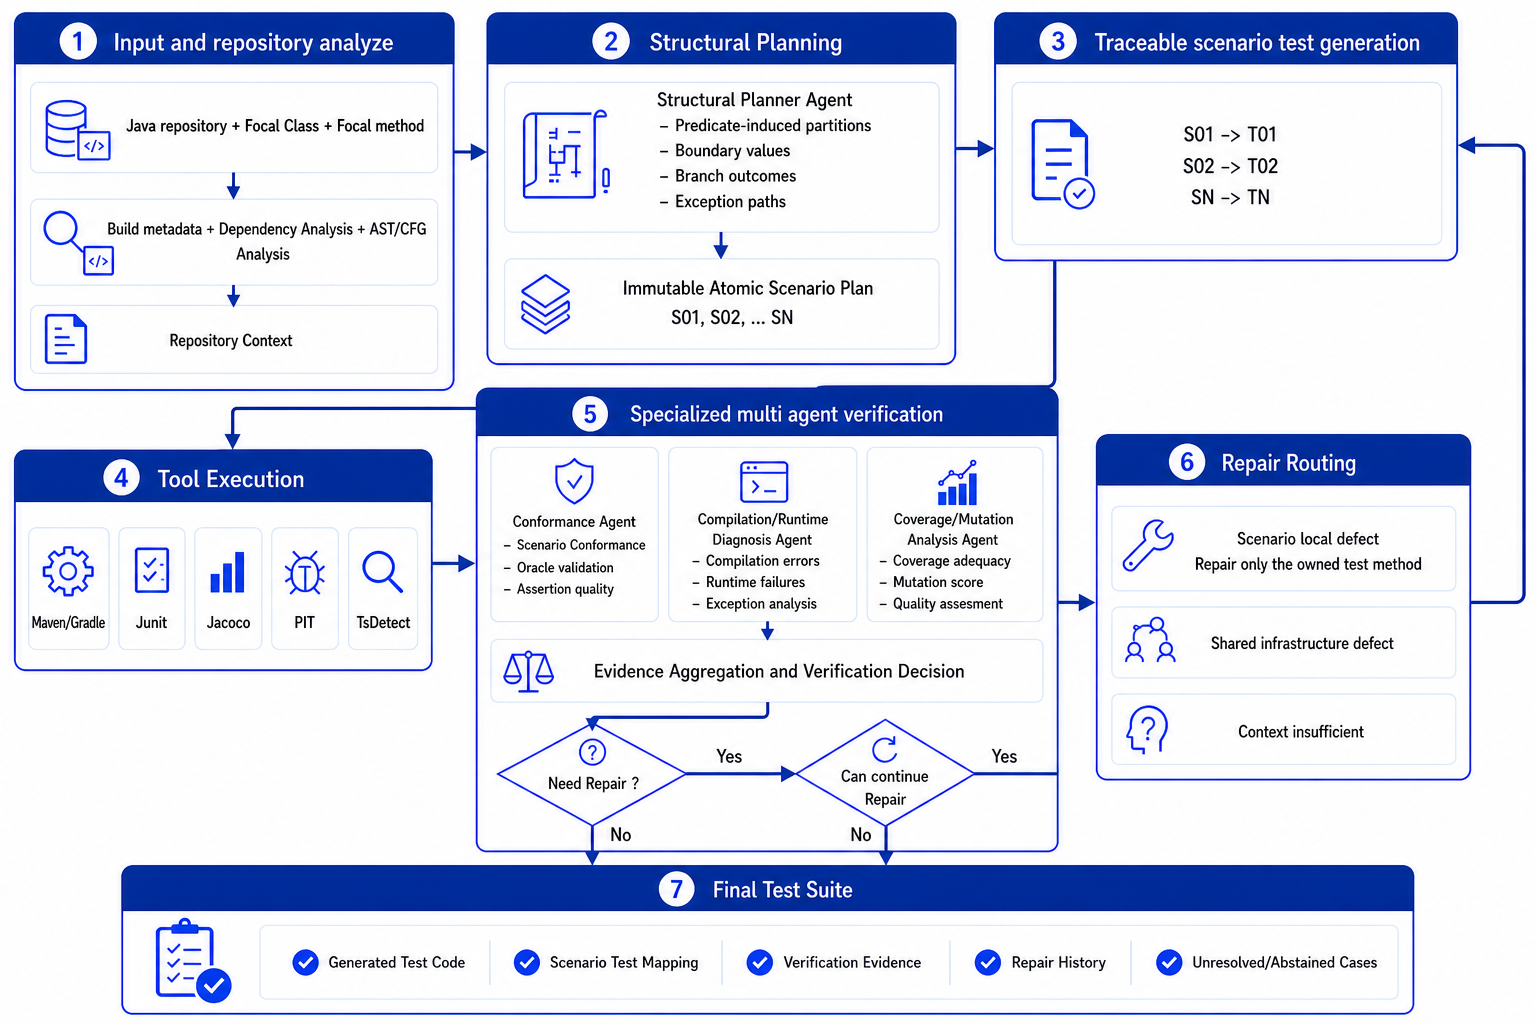
\includegraphics[width=\textwidth]{framework-pipeline-blue-v4-compact.png}
\caption{Overview of the TRACE framework.}\label{fig:trace-framework}
\end{figure}

The framework takes a Java repository, a focal class, a focal method, and a pipeline configuration file. The output includes accepted test code, scenario--test mapping, verification evidence, repair history, and unresolved or abstained cases. This design serves three research questions (Research Question-RQ): RQ1 separates the impact of Structural Planning from Direct Generation; RQ2 evaluates Traceability-Guided Scenario-Local Repair against Failing-Test-Method Repair and Full-Class Regeneration; RQ3 assesses Tool-Grounded Specialized Multi-Agent Verification compared to Basic Tool Gates and a General-Purpose Reviewer when methods receive the same tool evidence.

\subsection{Input analysis and repository}\label{subsec:input-analysis}

The first module builds a repository context to bind all decisions in the subsequent steps. TRACE identifies the Java version, build tool, module path, test framework, dependencies, source--test directory structure, Application Programming Interface (API) of the focal class, signature of the focal method, existing requirement/oracle sources, and related tests. Integrating the build, dependencies, and focal context into the pipeline is directly compatible with ChatUniTest and CATGen \cite{bib3,bib5}, while also being consistent with project-level experimental settings in recent studies \cite{bib2,bib11}.

The repository analysis function is represented as follows:

\begin{equation}
M = f_{\mathrm{analyze}}(R,c,m,Y)
\label{eq:repository-analysis}
\end{equation}

In which: R is the raw Java project repository, including source code, test code, build files, and the resources necessary for analyzing or executing the project.

c is the focal class selected in R; this is the class containing the behavior that the study wants to test. m is the focal method belonging to c; this is the target method that the Structural Planner analyzes and the generated tests are aimed at.

Y is the pipeline.yaml configuration file, containing input parameters, build environment, LLM, planning, generation, verification, repair, metric, output, and scenario selection policy. $f_{\mathrm{analyze}}$ is the repository analysis and normalization function. It combines data extracted from R, c, and m with the configuration in Y to create a unified input representation for the entire pipeline. M is the normalized repository context; M is the output of $f_{\mathrm{analyze}}$ and is the common metadata source for the Planner, Generator, tool layer, verification agents, and repair layer. In this study, the structure of M is determined as follows:

\begin{equation}
\begin{aligned}
M = (&\,\mathrm{java\_version},\mathrm{build\_tool},\mathrm{dependencies},\mathrm{test\_framework},\\
&\mathrm{source\_paths},\mathrm{test\_paths},\mathrm{focal\_class\_api},\\
&\mathrm{focal\_method\_signature},\mathrm{complexity\_map},\mathrm{existing\_tests},\\
&\mathrm{requirement\_evidence},\mathrm{build\_commands},\mathrm{ast\_model},\mathrm{cfg\_model},\\
&\mathrm{input\_config},\mathrm{repo\_config},\mathrm{build\_config},\mathrm{llm\_config},\mathrm{prompt\_config},\\
&\mathrm{planning\_config},\mathrm{generation\_config},\mathrm{verification\_config},\mathrm{repair\_config},\\
&\mathrm{metrics\_config},\mathrm{output\_config},\mathrm{report\_config})
\end{aligned}
\label{eq:repository-context}
\end{equation}

The groups \texttt{java\_version}, \texttt{build\_tool}, dependencies, \texttt{test\_framework}, \texttt{source\_paths}, \texttt{test\_paths}, \texttt{focal\_class\_api}, \texttt{focal\_method\_signature}, \texttt{complexity\_map}, \texttt{existing\_tests}, \texttt{requirement\_evidence}, and \texttt{build\_commands} are extracted or inferred from R, c, and m. Among them, \texttt{complexity\_map} stores structural features needed for selecting test targets; \texttt{focal\_class\_api} describes constructors, fields, and methods that generated tests can use; \texttt{requirement\_evidence} stores contracts/Javadoc, behaviors confirmed by existing tests, invariants observable in the repository, and the corresponding provenance; \texttt{build\_commands} are normalized Maven or Gradle commands for the target repository. When requirement/oracle sources in the repository are contradictory or insufficient, M records an indeterminate state instead of creating expected behavior without basis.

\texttt{ast\_model} is an Abstract Syntax Tree (AST) model, representing the tree form of a program's syntactic structure. \texttt{cfg\_model} is a Control-Flow Graph (CFG) model, in which nodes represent statements or basic blocks and edges represent possible control transfers. From the AST and CFG, TRACE collects predicates, predicate outcomes, branches, exceptional exits, and simple data dependencies of m to support Structural Planning. The \texttt{input\_config}, \texttt{repo\_config}, and \texttt{build\_config} groups describe the input, repository location, and build environment. \texttt{llm\_config} and \texttt{prompt\_config} describe the model, inference settings, and prompt template. \texttt{planning\_config}, \texttt{generation\_config}, \texttt{verification\_config}, and \texttt{repair\_config} define the budget and policy for the four corresponding stages; \texttt{planning\_config} also contains the test-method cap and scenario-selection policy that were fixed before execution. \texttt{metrics\_config} selects measures for coverage, mutation, and test smell; \texttt{output\_config} and \texttt{report\_config} define the artifacts and reports to be saved. These fields come from Y and do not change the meaning of the structured data extracted from R.

The output of the module is a repository-context object with structure, not a free-form prompt. As a result, the Planner uses structured facts; the Generator uses valid APIs, imports, and test frameworks; the tool layer uses the correct build command and path; and the repair layer reuses the same metadata to limit the scope of modifications.

\subsection{Auditable Structural Planning}\label{subsec:structural-planning}

The second module realizes the contribution C1---Auditable Test-Design-Technique-Grounded Structural Planning. Before generating test code, the Structural Planner Agent creates an immutable atomic scenario plan based on equivalence partitioning, boundary-value analysis, predicate-induced partition, branch outcome, and exception/error path. A predicate is a Boolean condition that governs control flow; a predicate-induced partition is the input domain divided according to the outcomes of that condition. These techniques are consistent with the role of test-design techniques in the International Organization for Standardization/International Electrotechnical Commission/Institute of Electrical and Electronics Engineers (ISO/IEC/IEEE) 29119-4:2021 standard \cite{bib6}.

The planning function is represented as follows:

\begin{equation}
\Pi = P_{\mathrm{struct}}(M,c,m) = \{S_i \mid 1 \leq i \leq n\}
\label{eq:structural-plan}
\end{equation}

Here, $P_{\mathrm{struct}}$ is the Structural Planning function; the function uses the repository context M and the focal target pair (c, m) to infer the plan \ensuremath{\Pi}. The symbol \ensuremath{\Pi} denotes the set of immutable atomic scenarios; n is the total number of scenarios in the plan; i is the index of the scenario, running from 1 to n; and $S_i$ is the i-th scenario. M, c, and m retain the meanings defined in Section~\ref{subsec:input-analysis}. Each atomic scenario $S_i$ is represented as follows:

\begin{equation}
\begin{aligned}
S_i = (&\,id_i, technique_i, trigger_i, input\_partition_i, expected\_behavior_i,\\
&oracle\_provenance_i, structural\_target_i, required\_context_i)
\end{aligned}
\label{eq:atomic-scenario}
\end{equation}

In the above tuple, \texttt{id\_i} is the stable identifier of the scenario; \texttt{technique\_i} records the test design technique that generated the scenario; \texttt{trigger\_i} is the activation condition; \texttt{input\_partition\_i} is the input class or boundary region from which values need to be taken; \texttt{expected\_behavior\_i} is the observable behavior that the oracle must check; \texttt{oracle\_provenance\_i} points to the requirement, contract/Javadoc, already verified test, or invariant serving as the basis for the expected behavior; \texttt{structural\_target\_i} is the line, branch, predicate outcome, or exception path that the scenario targets; \texttt{required\_context\_i} lists the fixture, object state, dependency, or exception condition needed to execute the scenario. A scenario without sufficiently reliable oracle provenance is marked as uncertain and must not be automatically accepted into the test suite.

Plan \ensuremath{\Pi} remains unchanged after release. If a step fails due to test implementation, TRACE fixes the implementation test $S_i$ rather than silently changing the scenario set. If evidence shows that the expected behavior is unfounded, oracle sources are conflicting, or the structural target is infeasible, the scenario is moved to the abstained/unresolved state with provenance instead of being corrected like a test defect. Therefore, the plan can be audited by counting and comparing equivalence classes, boundary values, branch outcomes, and exception paths before the test code is accepted. Unlike the Requirement Planner that derives test requirements from semantic analysis in TestAgent \cite{bib7}, the planning unit of TRACE is the structural target with oracle provenance and can be compared with Direct Generation under the same generation budget in RQ1.

\subsection{Traceable Scenario-Based Test Generation}\label{subsec:traceable-generation}

The third module implements the first part of the contribution C2-Bijective Scenario Ownership and Regression-Checked Scenario-Local Repair. For each $S_i$ in \ensuremath{\Pi}, TRACE generates exactly one test method $T_i$. This relationship prevents the Generator from mixing multiple independent scenarios into the same method or creating methods without a responsible scenario.

The test function according to the scenario is represented as follows:

\begin{equation}
T_i = G_{\mathrm{trace}}(S_i,M,\theta), \qquad 1 \leq i \leq n
\label{eq:trace-generation}
\end{equation}

In which, $G_{\mathrm{trace}}$ is the traceable scenario test generation function; $S_i$ is the source scenario; M is the repository context; \ensuremath{\theta} is the set of inference parameters of the LLM, such as model identifier, temperature, context limit, and generation limit; $T_i$ is the generated test method implementing $S_i$. The index i and the limit n retain the meaning from Section~\ref{subsec:structural-planning}.

Candidate test suite and scenario--test mapping are defined as follows:

\begin{equation}
T = \{T_i \mid 1 \leq i \leq n\}, \qquad
\Omega = \{(S_i,T_i) \mid 1 \leq i \leq n\}
\label{eq:scenario-test-mapping}
\end{equation}

In which, T is the set of candidate test methods and \ensuremath{\Omega} (Omega) is the set of scenario--test mapping pairs. \ensuremath{\Omega} is bijective within the generated suite: each $S_i$ maps to exactly one $T_i$ and each $T_i$ maps back to exactly one $S_i$; therefore |\ensuremath{\Pi}| = |T| = n.

Ownership invariant is recorded as follows:

\begin{equation}
\operatorname{owner}(T_i)=S_i \land \operatorname{implements}(T_i)=S_i
\label{eq:ownership-invariant}
\end{equation}

In this, owner is a function that returns the scenario owning $T_i$; implements is a function that returns the scenario that $T_i$ implements; and the symbol means that both conditions must be true simultaneously. $T_i$ stores \texttt{id\_i} in a machine-readable form, for example in the method name, annotation, structured comment, or sidecar mapping. The prompt generating $T_i$ only contains edit permissions for the method owned by $S_i$. \ensuremath{\Omega} therefore provides an attribution and repair unit smaller than the whole-file level \cite{bib2,bib3,bib9,bib10}.

\subsection{Tool Execution and Evidence Collection}\label{subsec:tool-execution}

The fourth module executes generated tests in the target repository and collects tool-grounded evidence. TRACE calls Maven or Gradle according to M, then runs tests using a framework compatible with the project, such as JUnit. If compilation is successful, the system collects execution results, stack traces, and assertion outcomes. For a valid run, TRACE collects branch/line coverage using Java Code Coverage (JaCoCo) and mutation evidence using PIT. tsDetect is run on the generated test file/class to collect test-smell evidence at the level reported by the detector. These tools support multi-dimensional evaluation rather than relying only on compilation pass/fail \cite{bib11,bib12,bib13}.

To attribute to each scenario, TRACE collects compile, run, assertion outcome, coverage, and mutation evidence for each pair ($S_i$, $T_i$) by running $T_i$ separately or using an equivalent test filtering mechanism; then the framework reruns the related test set to check interactions and regression. Since the default output of tsDetect is aggregated by test file, smell findings are stored as class/suite-level quality evidence and are not used alone to assign the primary failure cause for $S_i$. If an analysis implementation temporarily contains only $T_i$ along with the required scaffolding, the report must clearly specify the isolation procedure and provenance before the smell is linked to the scenario. When a measurement is unavailable due to build or tool limitations, the unavailable status is recorded instead of being inferred by an LLM.

The evidence record of the pair ($S_i$, $T_i$) is represented as follows:

\begin{equation}
\begin{aligned}
E_i = (&\,compile_i, run_i, assertion\_outcome_i, coverage_i, mutation_i,\\
&logs_i, provenance_i)
\end{aligned}
\label{eq:evidence-record}
\end{equation}

In which, $E_i$ only contains the observable evidence for scenario i: \texttt{compile\_i} stores the compilation state and compiler diagnostics; \texttt{run\_i} stores the execution state and runtime failure; \texttt{assertion\_outcome\_i} stores assertion pass/fail observed by the test runner but does not itself conclude whether the oracle is correct; \texttt{coverage\_i} records the achieved line/branch targets; \texttt{mutation\_i} records related mutants that were killed, survived, or not yet evaluated; \texttt{logs\_i} stores raw compiler messages, stack traces, and tool output; \texttt{provenance\_i} stores tool version, command, configuration, repository state, and report path. Scenario conformance, oracle validity, and assertion quality are not included in $E_i$ but are inferred by the Conformance Agent in the next module. The tsDetect test-smell report is stored separately at the class/suite scope as described above.

Tool execution is separated from LLM reasoning. With repository state, tool version, command, and fixed configuration, the tool provides measurements that can be reproduced under controlled conditions; agents in the subsequent module explain the evidence but are not allowed to replace missing evidence with speculation. Builds/tests that show flaky behavior or are environment-dependent are marked as uncertain and are not called deterministic. This distinction also does not assume that the behavior of the LLM is deterministic.

\subsection{Specialized Multi-Agent Verification}\label{subsec:specialized-verification}

The fifth module implements the C3 contribution---Tool-Grounded Specialized Multi-Agent Verification for Scenario-Level Failure Attribution. The Conformance Agent checks the relationship between $T_i$ and $S_i$, oracle provenance, and assertion quality without assuming that these conclusions are already present in the raw evidence. Compilation/Runtime Diagnosis Agents analyze compiler diagnostics, missing imports, dependency conflicts, runtime exceptions, fixture construction errors, and assertion failures. Coverage/Mutation Analysis Agents check structural-target satisfaction, branch contribution, and mutation evidence. Agents run in parallel when the corresponding evidence in $E_i$ is ready; agents without evidence are required to return unavailable/abstain instead of speculating.

The three agents generate the reports $V_{\mathrm{conf},i}$, $V_{\mathrm{run},i}$, and $V_{\mathrm{covmut},i}$. $V_{\mathrm{conf},i}$ is the report on scenario conformance, oracle validity, and assertion quality; $V_{\mathrm{run},i}$ is the compilation/runtime diagnosis report; $V_{\mathrm{covmut},i}$ is the coverage/mutation adequacy report. The reports retain their own evidence provenance so that the Evidence Aggregator can verify the agent's conclusions against the raw tool output. The Evidence Aggregator aggregates them using the following function:

\begin{equation}
D_i = f_{\mathrm{aggregate}}(S_i,T_i,E_i,V_{\mathrm{conf},i},V_{\mathrm{run},i},V_{\mathrm{covmut},i})
\label{eq:evidence-aggregation}
\end{equation}

In this, $f_{\mathrm{aggregate}}$ is the aggregation function according to a fixed decision schema; the function reconciles scenario, test, raw tool evidence, and three specialized reports. $D_i$ is the verification decision for scenario i, including acceptance status, primary failure cause, evidence provenance, confidence or uncertainty level, and proposed repair route. The schema prioritizes mandatory build/run gates; when these gates are achieved, the system then considers conformance/oracle and structural adequacy. If the reports conflict or required evidence is missing, the system does not select accept but moves to an appropriate indeterminate state. The symbols $S_i$, $T_i$, and $E_i$ retain the meanings defined in previous sections.

The route space includes accept, \texttt{repair\_scenario\_local}, \texttt{repair\_shared\_infrastructure}, and \texttt{abstain\_context\_insufficient}. Accept is only chosen when the required gates, scenario conformance, and oracle validity are all satisfied; \texttt{repair\_scenario\_local} is chosen when the error is due to the implementation of $T_i$; \texttt{repair\_shared\_infrastructure} is chosen when the error lies in a fixture, helper, dependency, or shared build configuration; \texttt{abstain\_context\_insufficient} is chosen when the evidence is insufficient, the oracle is conflicting, or the scenario/target cannot be safely verified. Therefore, a test that compiles successfully can still be rejected if $S_i$ is not implemented, the structural target is not touched, or the expected behavior is not checked. TestAgent had a Reviewer receiving execution, coverage, and mutation evidence \cite{bib7}, while MAGISTER separated the roles of analyzer/generator/executor/refiner \cite{bib8}; the difference of TRACE is maintaining independent specialized reports, attaching provenance to immutable scenario IDs, and synthesizing primary failure attribution along with the repair route. In RQ3, this design is compared with Basic Tool Gates and a General-Purpose Reviewer receiving the same tool evidence.

\subsection{Repair Routing and Scenario-Local Repair}\label{subsec:repair-routing}

The sixth module completes the C2 contribution by routing repair according to $D_i$. With scenario-local defect, TRACE only fixes or regenerates $T_i$ owned by $S_i$. Repair input includes $S_i$, $T_i$, M, $E_i$, $D_i$, and the relevant part of the tool log; the repair prompt does not allow rewriting test methods that are not owned and have been verified.

The local repair function is represented as follows:

\begin{equation}
T_i^{\prime} = f_{\mathrm{repair\_local}}(S_i,T_i,M,E_i,D_i,b_i)
\label{eq:local-repair}
\end{equation}

In which, $f_{\mathrm{repair\_local}}$ is the function to repair or regenerate a single method $T_i$ based on the scenario, repository context, evidence, and diagnosis; $b_i$ is the remaining repair budget of scenario i; $T_i^{\prime}$ is the repaired version of $T_i$, and the prime symbol \ensuremath{\prime} indicates a new candidate after a repair iteration. $S_i$, M, $E_i$, and $D_i$ retain the same definitions as in the previous sections. After the repair, TRACE compiles and reruns $T_i^{\prime}$, collects the target evidence, and then runs a regression check on previously verified tests that may be affected by class-level setup or shared fixtures. $T_i^{\prime}$ only replaces $T_i$ when the local fault is fixed and no previously verified test changes from pass to fail. The edit scope, number of iterations, token/API cost, repair success, and regression are recorded to answer RQ2.

With shared-infrastructure defects, TRACE switches to the shared repair procedure and reruns the entire affected scenario set; the defect is not incorrectly assigned to an individual $S_i$. For context-insufficient, oracle-conflict, or invalid-scenario cases, the system abstains and records the case as unresolved along with a reason code and provenance instead of continuing to ask the LLM to guess repository information or modify the test to match an unreliable scenario. Plan \ensuremath{\Pi} is not changed in the current run; any future plan edits must create a new version and cannot be considered scenario-local repair. Each round stops when a candidate is accepted, $b_i$ is exhausted, or the route requests abstention.

\subsection{Final Test Suite and linkage with evaluation}\label{subsec:final-suite}

The seventh module packages the final output according to the expression:

\begin{equation}
A = (T_{\mathrm{final}},\Omega_{\mathrm{final}},E_{\mathrm{final}},H_{\mathrm{repair}},U_{\mathrm{abstain}})
\label{eq:final-artifact}
\end{equation}

In which, A is the final artifact package; $T_{\mathrm{final}}$ is the set of accepted test methods; $\Omega_{\mathrm{final}}$ is the scenario--test mapping that is still valid; $E_{\mathrm{final}}$ is the final set of verification evidence; $H_{\mathrm{repair}}$ is the repair history, including edit scope, iteration, and regression results; $U_{\mathrm{abstain}}$ is the set of unresolved or abstained scenarios along with the reason and evidence provenance. No unaccepted tests are included in $T_{\mathrm{final}}$.

This output is directly linked to the experimental design. RQ1 compares Structural Planning with Direct Generation under the same LLM, repository context M, generated-method cap, and generation budget by compilation/execution success, structural-target satisfaction, focal-method branch coverage, and mutation score. If |\ensuremath{\Pi}| exceeds the cap, the \texttt{planning\_config} in Y applies the scenario-selection policy that was fixed before running; both selected and omitted scenario IDs are recorded, and the Generators of both treatments receive the same method cap and generation budget. Planning cost is recorded separately so as not to be mixed with the generation budget. RQ2 compares Traceability-Guided Scenario-Local Repair with Failing-Test-Method Repair and Full-Class Regeneration from the same initial failing artifacts, $E_i$, LLM, and repair budget measured by token/API cost, edit scope, repair iteration, regression, repair success, and final test adequacy. RQ3 compares $f_{\mathrm{aggregate}}$ and specialized agents with Basic Tool Gates and General-Purpose Reviewer using false acceptance, scenario-level failure attribution, and primary repair-route accuracy.

By releasing an auditable plan \ensuremath{\Pi}, maintaining the bi-directional \ensuremath{\Omega}, storing raw evidence $E_i$ separately from agent inference, and only accepting repairs after regression checks, TRACE transforms LLM-based unit-test generation into a traceable workflow. The framework does not consider compilation success or the convincing commentary of the LLM as sufficient; the planned scenario, oracle provenance, generated method, tool evidence, verification decision, and regression result must be consistent before a test is included in $T_{\mathrm{final}}$. Test-smell evidence from tsDetect is kept within the scope that the detector actually reports and is not inferred into scenario-level attribution if isolation provenance is missing.



\section{Experiments and Results}\label{sec:experiments}

This section presents the experimental design used to evaluate the three main contributions of the proposed method. Three research questions are identified as follows:

RQ1 -- The effectiveness of Structural Planning.

Under the conditions of using the same LLM, repository context, limits on the number of generated test methods, and generation budget, how does Structural Planning based on test-design techniques affect compilation/execution success, structural-target satisfaction, focal-method branch coverage, and mutation score compared to Direct Generation without planning?

RQ2 -- Effectiveness of Traceability-Guided Scenario-Local Repair.

With the same initial failing scenario--test artifacts, tool evidence, LLM, and repair budget, does Traceability-Guided Scenario-Local Repair help reduce token/API cost, edit scope, number of repair iterations, and regressions on previously verified tests, while still maintaining repair success and final test adequacy, compared to Failing-Test-Method Repair without scenario context and Full-Class Regeneration?

RQ3 -- Accuracy of Tool-Grounded Specialized Multi-Agent Verification.

Compared to Basic Tool Gates and a General-Purpose Reviewer provided with tool evidence, how accurately can Tool-Grounded Specialized Multi-Agent Verification detect false acceptance, perform scenario-level failure attribution, and select the primary repair route?

RQ1 evaluates the impact of the structured planning step before test code generation. RQ2 evaluates the ability to use scenario--test traceability relationships to limit the scope of repair and protect the tests that have been verified. RQ3 Evaluate the mechanism of verifying multiple specialized agents in synthesizing tool evidence, detecting invalid artifacts, and correctly identifying the cause as well as the repair direction.

\subsection{Experimental design}\label{subsec:experimental-design}

The study conducted three experiments corresponding to three research questions, with each experiment using a separate dataset. Each run was performed on an independent workspace at a fixed repository revision. The build configuration, prompt, model, toolchain, and output artifacts were saved to support verification and replication. Maven/Gradle, JUnit, JaCoCo, and PIT respectively provided evidence for compilation, execution, coverage, and mutation testing.

For RQ1, DIRECT and PLANNED were compared using a paired design on the same 150 focal methods from 58 Java projects in SF110. DIRECT generates tests directly from the repository context, whereas PLANNED creates atomic scenarios from AST/CFG before generating tests. In each model configuration, both treatments used the same focal methods, source revision, repository context, decoding settings, a maximum limit of six generated test methods, and generation budget; repair and verifier feedback were disabled. Structural-Target Satisfaction of both was calculated on the same reference target set, determined independently before test generation. The experiment used Gemini 3.7 Flash and DeepSeek V4 Flash; each focal method--model--treatment combination was run once, resulting in a total of 600 runs (150 focal methods \ensuremath{\times} two models \ensuremath{\times} two treatments). Planning costs are recorded separately and included in the total costs of PLANNED.

For RQ2, TGSLR, FTMR, and FCR were evaluated on the same 100 initial failing artifacts across six LIBRO--Defects4J projects. The treatments used the same repository state, failure evidence, model, seed, repair budget, and stopping conditions. TGSLR received scenario--test mapping and only fixed the corresponding test method; FTMR fixed the same method but without scenario context; FCR was allowed to regenerate the entire test class. Each treatment ran once on each unit using the gemini 3.6 flash model, generating a total of 300 logic runs, with up to three repair rounds and budget. 75,000 tokens per run. The budget is checked between completed calls, so the last call may cause the total tokens to exceed the threshold; provider retries are not counted as a new experimental unit.

For RQ3, B0, B1, and B2 were evaluated on a separate verification dataset consisting of 73 cases from 14 Java projects, including 65 controlled-injection cases and eight natural cases. B0 only used compilation and selected-JUnit outcomes; B1 and B2 received the same evidence envelope, in which B2 used three specialized verifiers and an Evidence Aggregator. Providing the same evidence does not imply equal reasoning budgets; the number of calls and token counts were recorded to assess the cost trade-offs. Since the gold set was labeled with AI assistance and the cohort had been exposed to a previous prototype, RQ3 is considered an exploratory experiment.

\subsection{Measurement and analysis methods}\label{subsec:measurement}

RQ1 uses Compilation Success Rate, Execution Success Rate, Structural-Target Satisfaction, focal-method Branch Coverage, and Mutation Score. In the end-to-end analysis, tests that do not compile or do not execute receive a value of 0 for structural metrics. A supplementary analysis on the pairs that both execute successfully is used to evaluate conditional quality. Cost is measured by token usage and wall-clock time.

RQ2 uses core repair success, token/API cost, number of repair rounds, Changed LOC, and regression-producing repair attempts. A core repair is considered successful if it is applied, compiles, makes the focal test pass on the fixed revision, exhibits bug-revealing behavior on the buggy revision if needed, and does not leave any regression. Coverage and mutation are only reported descriptively on successful repairs with measurement evidence. Since the data does not yet have independent scenario conformance and structural-target satisfaction, RQ2 does not evaluate the entire acceptance contract of the framework. RQ3 uses decision accuracy, False-Acceptance Rate, False-pass F1, attribution Macro-F1, repair-route accuracy, coverage, and selective accuracy. Invalid output and abstention are reported separately instead of being considered correct decisions. Cost is measured by token usage and number of agent calls.

The McNemar exact test is used for binary outcomes; the Wilcoxon signed-rank test is used for paired continuous metrics. Results are reported along with effect size, 95\% bootstrap confidence interval, and Holm correction for the main testing groups. Because each unit--treatment is mainly run only once and the data is clustered by project, the results are limited to the evaluated configurations.

\subsection{RQ1 Results: The Impact of Structural Planning}\label{subsec:rq1}

This section presents the results of RQ1 to evaluate the impact of Structural Planning on the reliability, test adequacy, and cost of the unit test generation process. Two approaches were compared: DIRECT, in which the LLM generates tests directly from the repository context, and PLANNED, in which the LLM constructs a structural planning consisting of atomic scenarios before generating test code. The experiments used Gemini 3.7 Flash and DeepSeek V4 Flash on the same 150 focal methods from 58 projects for each model--approach combination, totaling 600 generation runs. Within each model configuration, both approaches used the same focal methods, source revision, repository context, decoding settings, a maximum limit of 6 generated test methods, and generation budget. Adaptive Repair was turned off so that the results directly reflect the quality of the initial generation.

According to the end-to-end scoring protocol, a run with an invalid test artifact, or one that does not compile or execute successfully, receives a value of 0 for Structural-Target Satisfaction (STS), Branch Coverage (BC), and Mutation Score (MS). This calculation simultaneously reflects the reliability of the test-generation pipeline and the adequacy of the generated test suite. N/A is only used when a metric is undefined due to the absence of a structural target or a valid denominator; these values are excluded from the calculation of the corresponding metric. DIRECT and PLANNED are paired by focal method, and statistical analysis is performed separately for each LLM.

\subsubsection{Descriptive Results}\label{subsubsec:rq1-descriptive}

\begin{table}[htbp]
\caption{END-TO-END DESCRIPTION RESULTS}\label{tab:rq1-descriptive}
\centering
\scriptsize
\begin{tabularx}{\textwidth}{@{}>{\raggedright\arraybackslash}X l r r r r r@{}}
\toprule
Model & Treatment & CSR, n (\%) & ESR, n (\%) & STS (\%) & BC (\%) & MS (\%) \\
\midrule
Gemini 3.7 Flash & DIRECT & 142 (94,67\%) & 124 (82,67\%) & 46,54 & 59,34 & 54,91 \\
Gemini 3.7 Flash & PLANNED & 147 (98,00\%) & 135 (90,00\%) & 58,38 & 71,19 & 64,32 \\
DeepSeek V4 Flash & DIRECT & 95 (63,33\%) & 50 (33,33\%) & 25,09 & 28,64 & 27,94 \\
DeepSeek V4 Flash & PLANNED & 142 (94,67\%) & 130 (86,67\%) & 58,57 & 69,98 & 63,52 \\
Aggregate & DIRECT & 237 (79,00\%) & 174 (58,00\%) & 35,52 & 43,51 & 41,43 \\
Aggregate & PLANNED & 289 (96,33\%) & 265 (88,33\%) & 58,47 & 70,58 & 63,92 \\
\bottomrule
\end{tabularx}
\end{table}

CSR: Compilation Success Rate; ESR: Execution Success Rate; STS: Structural-Target Satisfaction; BC: focal-method Branch Coverage; MS: focal-method Mutation Score. CSR and ESR have N = 150 for each model--approach combination. STS, BC, and MS are averages over non-N/A observations. For Gemini, the number of STS/BC/MS observations is 140/139/150 for both approaches; for DeepSeek, the corresponding numbers are 148/148/150 in DIRECT and 141/140/150 in PLANNED. The summary rows only provide aggregate descriptions and should not be used to infer or rank the two LLMs. Across both model configurations, PLANNED achieved a CSR of 96.33\%, 17.33 percentage points higher than DIRECT's 79.00\%. ESR increased from 58.00\% to 88.33\%, corresponding to 91 additional generated test suites executing successfully. For structural-adequacy metrics, STS increased from 35.52\% to 58.47\%, BC from 43.51\% to 70.58\%, and MS from 41.43\% to 63.92\%. These aggregated results show a consistent trend, but are only descriptive.

On Gemini 3.7 Flash, PLANNED improved all five metrics: CSR increased by 3.33 percentage points, ESR by 7.33 percentage points, STS by 11.84 percentage points, BC by 11.85 percentage points, and MS by 9.41 percentage points. The increases on DeepSeek V4 Flash were larger, at 31.34, 53.34, 33.48, 41.34, and 35.58 percentage points, respectively. Overall, Structural Planning is associated with more generated test suites passing the compilation/execution gates and satisfying more structural targets.

\subsubsection{Paired Statistical Analysis}\label{subsubsec:rq1-paired}

Because DIRECT and PLANNED are evaluated on the same focal methods, statistical analysis follows a paired design. The two-sided exact McNemar test is used for CSR and ESR. The two-sided Wilcoxon signed-rank test is used for STS, BC, and MS on the PLANNED - DIRECT differences, with tie correction, zero differences removed, and no continuity correction applied. Holm correction is applied for the family of five primary metrics within each LLM, with \ensuremath{\alpha} = 0.05. Matched odds ratio (OR) is reported for binary metrics, while paired rank-biserial correlation ($r_{\mathrm{rb}}$) is used for continuous metrics.

\begin{table}[htbp]
\caption{RESULTS OF PAIRED TESTS}\label{tab:rq1-paired}
\centering
\scriptsize
\begin{tabular}{@{}llllll@{}}
\toprule
Model & Metric & n & p & $p_{\mathrm{Holm}}$ & Effect size \\
\midrule
Gemini 3.7 & CSR & 150 & 0,0625 & 0,0625 & OR = $\infty$ (5/0) \\
Gemini 3.7 & ESR & 150 & 0,000977 & 0,001953 & OR = $\infty$ (11/0) \\
Gemini 3.7 & STS & 140 & $7,04\times10^{-6}$ & $2,11\times10^{-5}$ & $r_{\mathrm{rb}}=0,907$ \\
Gemini 3.7 & BC & 139 & $2,42\times10^{-7}$ & $1,21\times10^{-6}$ & $r_{\mathrm{rb}}=1,000$ \\
Gemini 3.7 & MS & 150 & $7,88\times10^{-7}$ & $3,15\times10^{-6}$ & $r_{\mathrm{rb}}=1,000$ \\
DeepSeek V4 & CSR & 150 & $5,52\times10^{-12}$ & $1,10\times10^{-11}$ & OR = 16,667 (50/3) \\
DeepSeek V4 & ESR & 150 & $3,43\times10^{-23}$ & $1,72\times10^{-22}$ & OR = 81,000 (81/1) \\
DeepSeek V4 & STS & 141 & $1,44\times10^{-10}$ & $1,44\times10^{-10}$ & $r_{\mathrm{rb}}=0,906$ \\
DeepSeek V4 & BC & 140 & $1,92\times10^{-13}$ & $5,76\times10^{-13}$ & $r_{\mathrm{rb}}=0,953$ \\
DeepSeek V4 & MS & 150 & $1,03\times10^{-14}$ & $4,13\times10^{-14}$ & $r_{\mathrm{rb}}=0,984$ \\
\bottomrule
\end{tabular}
\end{table}

n is the number of complete pairs before removing zero differences in the Wilcoxon test. CSR, ESR, and MS each have 150 pairs in each LLM; STS/BC have 140/139 pairs on Gemini and 141/140 pairs on DeepSeek. The numbers in parentheses after OR are respectively the number of pairs where PLANNED succeeded--DIRECT failed and the number of pairs in the opposite direction. OR = \ensuremath{\infty} indicates that there are no pairs in the opposite direction in the sample, which does not mean infinite effectiveness. $r_{\mathrm{rb}}$ > 0 favors PLANNED; $r_{\mathrm{rb}}$ = 1 indicates that all non-zero paired differences are positive.

After Holm correction, Gemini 3.7 Flash achieved statistically significant improvements in ESR, STS, BC, and MS; CSR did not reach the significance threshold ($p_{\mathrm{Holm}}$ = 0.0625). With DeepSeek V4 Flash, all five metrics reached statistical significance. The effect sizes for STS, BC, and MS were 0.907; 1.000; 1.000 on Gemini and 0.906; 0.953; 0.984 on DeepSeek, indicating that the paired differences mostly favored PLANNED. However, these tests used the focal method as the unit of analysis and have not adjusted for project clustering.

\subsubsection{Conditional Quality Analysis}\label{subsubsec:rq1-conditional}

End-to-end scoring combines pipeline reliability with the adequacy of the generated test suite. Since PLANNED has a higher ESR, the increase in STS, BC, and MS may partly come from the reduction of unsuccessful runs scored 0. Therefore, a secondary analysis was conducted on the focal methods that both DIRECT and PLANNED successfully executed. This is an exploratory available-pair analysis; the p-values have not been subjected to Holm correction and do not replace the primary end-to-end analysis. On Gemini, PLANNED increased STS by 9.70 percentage points (n = 114, p = 0.000208, $r_{\mathrm{rb}}$ = 0.863), BC by 7.83 percentage points (n = 113, p = $1.78\times 10^{-5}$, $r_{\mathrm{rb}}$ = 1.000), and MS by 6.25 percentage points (n = 124, p = $5.91\times 10^{-5}$, $r_{\mathrm{rb}}$ = 1.000).

On DeepSeek, the paired differences were smaller: STS increased by 1.18 percentage points (n = 47, p = 0.528, $r_{\mathrm{rb}}$ = 0.286), BC increased by 1.92 percentage points (n = 47, p = 0.293, $r_{\mathrm{rb}}$ = 0.476), and MS increased by 2.57 percentage points (n = 49, p = 0.0431, $r_{\mathrm{rb}}$ = 1.000). Only MS reached the 0.05 threshold before multiple-testing correction; this result would no longer reach the threshold if applying Holm correction for the three conditional metrics. The analysis by paired-executed subjects therefore does not support the previous assertion that conditional MS of PLANNED is lower: the comparison of 83.82\% versus 73.29\% was based on two sets of successful runs with different sizes and not a paired comparison. Evidence of executable-suite adequacy is generally clear on Gemini but remains limited on DeepSeek.

\subsubsection{Costs and Trade-offs (Cost Trade-off)}\label{subsubsec:rq1-cost}

Structural Planning uses an additional LLM phase to create a plan, which increases costs. On Gemini, the mean wall-clock time increased from 13.45 s to 18.95 s (+40.92\%), while mean token usage increased from 3,750 to 7,450 tokens per run; total tokens increased from 562,500 to 1,117,500 (+98.67\%). On DeepSeek, the mean wall-clock time increased from 64.34 s to 100.06 s (+55.54\%), while mean token usage increased from 7,904.10 to 16,189.38 tokens; total tokens increased from 1,185,615 increased to 2,428,407 (+104.82\%). Meanwhile, the average number of generated test methods decreased from 3.65 to 2.92 on Gemini and from 5.74 to 2.92 on DeepSeek. Thus, the end-to-end improvement does not come from generating more test methods, but it comes with nearly double the token consumption and higher wall-clock time.

\subsubsection{Answer to RQ1}\label{subsubsec:rq1-answer}

Among the two evaluated model configurations, PLANNED statistically significantly improves ESR, STS, BC, and MS after Holm correction; CSR only reaches statistical significance on DeepSeek. Primary results indicate that Structural Planning improves pipeline reliability and end-to-end test adequacy. Secondary paired-executed analysis shows that adequacy benefits are still clear on Gemini, but weak and unstable on DeepSeek. Therefore, the data does not yet support a generalized conclusion that PLANNED always produces stronger executable test suites than DIRECT across all LLMs. The achieved benefits also come with nearly double the token usage and higher wall-clock time. This is an ablation study aimed at isolating the influence of planning; each configuration only has one run per focal method, and the tests have not yet accounted for project clustering or between-run variability. Therefore, the conclusion is limited to the dataset, model configurations, and budget that were examined.

\subsection{RQ2 Results: Effectiveness of Traceability-Guided Scenario-Local Repair}\label{subsec:rq2}

\subsubsection{RQ2 Experimental Setup}\label{subsubsec:rq2-setup}

RQ2 compares Traceability-Guided Scenario-Local Repair (TGSLR), Failing-Test-Method Repair without scenario context (FTMR), and Full-Class Regeneration (FCR) on the same original faulty unit and tool outputs. The treatments use the same repository, model, budget, seed, and stopping conditions. TGSLR receives failure evidence along with scenario--test traceability and only repairs the test method that owns the scenario; FTMR receives the same failure evidence but without scenario/traceability; FCR is allowed to regenerate the test class.

The dataset consists of 100 distinct fault units from six LIBRO--Defects4J projects and 300 logic runs using models/gemini-3.6-flash. Each treatment is run once on each unit with seed 20260814, a 75,000-token budget, and a maximum of three repair rounds. Since the budget is checked between completed calls, the last call may exceed the limit; provider retries do not create new experimental units.

All 100 pairs were retained; all other results of Success---including two Cancelled runs of D4J-JACKSONXML-4-25 and one Unexpected run of FTMR---were failures. Exact McNemar was used for success and regression; paired Wilcoxon was used for tokens, API call counts, and the number of revision rounds. Holm adjusted ten tests from two comparisons \ensuremath{\times} five outcomes. The study reported matched odds ratio or paired rank-biserial correlation along with unadjusted 95\% paired bootstrap CI (10,000 resamples; seed 20260814). The number of changed lines and adequacy were only described because different subsets for success or measurements according to treatment were used.

\subsubsection{Core Repair Success and Paired Comparison}\label{subsubsec:rq2-success}

The Success status in CSV requires the candidate to be applicable, compiled, and pass the focal test successfully on the fixed revision, the bug can be reproduced on the buggy revision when necessary, and no regression is caused. Since CSV does not have a scenario conformance or structural target field, this outcome only measures core repair, not the entire acceptance contract of TRACE; coverage and mutation are reported separately.

\begin{table}[htbp]
\caption{Core repair success per 100 defect units of each treatment.}\label{tab:rq2-core-success}
\begin{tabular}{@{}lrrr@{}}
\toprule
Repair strategy & Runs & Successful core repairs & Core repair success rate \\
\midrule
TGSLR & 100 & 60 & 60,0\% \\
FTMR & 100 & 46 & 46,0\% \\
FCR & 100 & 76 & 76,0\% \\
\bottomrule
\end{tabular}
\end{table}

TGSLR succeeded 60/100 runs, compared to 46/100 for FTMR and 76/100 for FCR. The number of focal test passes were 72, 73, and 93, respectively; the number of buggy-revision oracle passes were 66, 52, and 84. It is not possible to report the compile rate separately because the CSV only records this result in the status/stop reason.

\begin{table}[htbp]
\caption{Comparison of paired core repair success.}\label{tab:rq2-paired-success}
\centering
\scriptsize
\begin{tabularx}{\textwidth}{@{}>{\raggedright\arraybackslash}X r *{4}{>{\centering\arraybackslash}X}@{}}
\toprule
Comparison & Pairs & TGSLR success & Comparator success & Difference & TGSLR win/tie/loss \\
\midrule
TGSLR--FTMR & 100 & 60,0\% & 46,0\% & +14.0 percentage points & 21/72/7 \\
TGSLR--FCR & 100 & 60,0\% & 76,0\% & -16.0 percentage points & 4/76/20 \\
\bottomrule
\end{tabularx}
\end{table}

For TGSLR--FTMR, W/T/L = 21/72/7, matched odds ratio = 3.00 (95\% CI: 1.23--8.35) and $p_{\mathrm{Holm}}$ = 0.0752; the 14-point advantage is therefore only descriptive after adjustment. For TGSLR--FCR, W/T/L = 4/76/20, matched odds ratio = 0.20 (95\% CI: 0.05--0.60) and $p_{\mathrm{Holm}}$ = 0.0108, confirming that FCR has a higher core repair success.

\subsubsection{LLM costs, number of revisions, and scope of edits}\label{subsubsec:rq2-cost}

\begin{table}[htbp]
\caption{Costs, number of repair cycles, and number of lines changed.}\label{tab:rq2-cost}
\centering
\scriptsize
\begin{tabularx}{\textwidth}{@{}l *{4}{>{\centering\arraybackslash}X}@{}}
\toprule
Repair strategy & Mean tokens per run & Mean API calls per run & Mean repair iterations per run & Mean changed LOC per successful repair \\
\midrule
TGSLR & 25.284,9 & 4,51 & 2,05 & 18,4 \\
FTMR & 28.238,2 & 4,82 & 2,30 & 16,5 \\
FCR & 17.798,2 & 3,74 & 1,39 & 28,9 \\
\bottomrule
\end{tabularx}
\end{table}

Compared to FTMR, TGSLR has a lower average value of 2,953.3 tokens, 0.31 API calls, and 0.25 edit rounds per run, but no difference is significant after Holm: $p_{\mathrm{Holm}}$ = 0.1830, 0.7089, and 0.0912; rank-biserial correlation is -0.230, 0.152, and 0.397; 95\% CI of FTMR-TGSLR is [96.7; 6,125.0], [-0.39; 0.98], and [0.04; 0.46]. Compared with FCR, TGSLR used 7,486.7 more tokens, 0.77 more API calls, and 0.66 more repair iterations; the corresponding $p_{\mathrm{Holm}}$ values were $3.82\times 10^{-6}$, 0.00185, and $5.49\times 10^{-7}$; the rank-biserial correlations were 0.585, 0.470, and 0.754; and the 95\% CIs were [4,974.2; 10,153.9], [0.26; 1.27], and [0.46; 0.86]. Among successful repairs, TGSLR changed an average of 18.45 lines, compared with 16.50 for FTMR and 28.93 for FCR; the increase of 1.95 lines and decrease of 10.48 lines are descriptive only because the sets of successful repairs differ.

\subsubsection{Regression and final test adequacy}\label{subsubsec:rq2-regression}

\begin{table}[htbp]
\caption{Regression over the entire run and adequacy on successful repairs with measurements.}\label{tab:rq2-regression}
\centering
\scriptsize
\begin{tabularx}{\textwidth}{@{}l *{5}{>{\centering\arraybackslash}X}@{}}
\toprule
Repair strategy & Runs with regression & Coverage measurements / successful repairs & Mean line coverage & Mutation measurements / successful repairs & Mean mutation score \\
\midrule
TGSLR & 6 & 51/60 & 34,4\% & 40/60 & 17,6\% \\
FTMR & 6 & 39/46 & 31,3\% & 29/46 & 14,6\% \\
FCR & 8 & 59/76 & 37,9\% & 47/76 & 18,7\% \\
\bottomrule
\end{tabularx}
\end{table}

TGSLR and FTMR both recorded six regression events (preserving 94\% of protected tests), compared to eight for FCR (92\%); both pairwise comparisons were not significant after correction ($p_{\mathrm{Holm}}$ = 1.000). For the available successful repair measures, the average line coverage and mutation score of TGSLR were higher than FTMR but lower than FCR. The outcomes ToolFailed, ReportMissing, and NotRun were considered as missing rather than 0, so adequacy was only interpreted descriptively.

\subsubsection{Answering RQ2}\label{subsubsec:rq2-answer}

RQ2 is partially supported. Compared with FTMR, TGSLR achieved higher core repair success and lower mean cost, but none of the paired differences remained significant after Holm correction; successful TGSLR patches also changed 1.95 more lines on average. Compared with FCR, successful TGSLR patches changed 10.48 fewer lines and TGSLR recorded two fewer regression events, but FCR achieved significantly higher success and lower cost; the regression difference was not significant. Thus, TGSLR exhibits a descriptive trade-off in locality rather than overall superiority. The evidence comes from one run per treatment, one model, and six clustered projects. The CSV lacks an independent compilation outcome, repair time, scenario conformance, structural target, and oracle strength; therefore, the results do not establish causality or the full TRACE acceptance contract.

\subsection{RQ3 Results: Evaluation of Tool-Grounded Specialized Multi-Agent Verification}\label{subsec:rq3}

RQ3. Compared with the Basic Tool Gate (B0) and a General-Purpose Reviewer using the same tool evidence (B1), how accurately does the Specialized Multi-Agent Verifier (B2) control false acceptance, attribute causes, and select the primary repair route?

\subsubsection{Design and scope of reasoning}\label{subsubsec:rq3-design}

This is an exploratory v2 evaluation of 73 cases across 14 Java projects, including 65 controlled-injection cases and 8 natural cases. The gold set was built following an AI-assisted process with the involvement of a human annotator. Two independent annotation rounds were conducted through two separate calls to DeepSeek Reasoner on 180 candidate cases. Both rounds only received public cases, test source, candidate focal-class source, static mapping evidence, and scenario card; they were blind to B0/B1/B2 outputs, private gold category, injection operator, repair route, and validation label.

Across 180 cases, the two AI passes agreed on the mapping decision in 149 cases (82.78\%; Cohen's \ensuremath{\kappa} = 0.460). This is AI inter-pass agreement, not agreement between human annotators. Because the study had only one human annotator, human inter-rater agreement could not be calculated. The final cohort comprised 73 cases for which both AI passes confirmed the mapping and agreed on a compatible focal class and method; therefore, the 73/73 agreement is a consequence of the cohort-selection criterion, not an independent reliability estimate.

Disagreements about mapping decisions, focal class, or incompatible methods are excluded from the cohort. For cases requiring additional review, a human annotator performs the final adjudication without using the outputs of B0, B1, or B2. The protocol initially planned a third blind LLM pass for disagreements related only to scenario type, but the current artifact does not store a separate third-pass field; instead, the results were reviewed by a human annotator before confirming the final cohort.

AI participates in suggesting and checking mapping/scenario, while also evaluating mutant relevance in weak-oracle cases. A human annotator is responsible for reviewing and confirming the final results. Gold decision, cause, and repair route are deterministically mapped from the frozen category along with tool/injection evidence. Since there is only one human annotator and no independent evaluation by a second annotator, the results are interpreted as exploratory evidence.

B0 uses compilation and selected-JUnit results. B1 is a general reviewer. B2 consists of three specialists in plan-to-test conformance, compilation/runtime, and coverage/mutation; a deterministic aggregator creates the decision, primary cause, and repair route. In each case, B1 and B2 receive an evidence envelope with the same SHA-256. The cohort has 26 false-passing cases and 54 cases with the gold decision \texttt{REPAIR\_REQUIRED}.

\begin{table}[htbp]
\caption{Safety and quality outcome measures}\label{tab:rq3-safety}
\centering
\scriptsize
\begin{tabularx}{\textwidth}{@{}>{\raggedright\arraybackslash}X l *{5}{>{\centering\arraybackslash}X}@{}}
\toprule
Model/run & Verifier & False-pass F1 & FAR & Decision accuracy & Coverage & Selective accuracy \\
\midrule
Overall & B0 & 0.00\% & 100.00\% & 45.21\% & 100.00\% & 45.21\% \\
Gemini 3.5 & B1 & 59.46\% & 57.69\% & 60.27\% & 100.00\% & 60.27\% \\
Gemini 3.5 & B2 & 64.00\% & 26.92\% & 65.75\% & 82.19\% & 70.00\% \\
DeepSeek (repaired) & B1 & 70.00\% & 42.31\% & 72.60\% & 87.67\% & 71.88\% \\
DeepSeek (repaired) & B2 & 70.00\% & 0.00\% & 61.64\% & 76.71\% & 80.36\% \\
GLM sensitivity & B1 & 20.69\% & 3.85\% & 57.53\% & 46.58\% & 94.12\% \\
GLM sensitivity & B2 & 26.67\% & 0.00\% & 47.95\% & 60.27\% & 77.27\% \\
\bottomrule
\end{tabularx}
\end{table}

Gemini produced consistently favorable point estimates for B2: detecting 16/26 false-passing cases instead of 11/26, reducing false acceptance from 15 to 7 cases, and increasing selective accuracy by 9.73 percentage points; in return, B2 generated 8 false positives and abstained on 13 cases. On the DeepSeek repaired set, B2 eliminated 11 false acceptances, but Decision Accuracy decreased by 10.96 points due to lower coverage. GLM also reduced FAR, but had 87 invalid outputs (B1: 37; B2: 50), so it cannot be used to claim superiority.

\subsubsection{Attribution, routing and uncertainty}\label{subsubsec:rq3-routing}

\begin{table}[htbp]
\caption{Diagnosis and repair routing on 54 REPAIR\_REQUIRED cases}\label{tab:rq3-routing}
\centering
\scriptsize
\begin{tabularx}{\textwidth}{@{}>{\raggedright\arraybackslash}X l *{3}{>{\centering\arraybackslash}X}@{}}
\toprule
Model/run & Verifier & Attribution Macro-F1 & Routing accuracy & Abstention \\
\midrule
Overall & B0 & 7.35\% & 31.48\% & 0.00\% \\
Gemini 3.5 & B1 / B2 & 35.21\% / 37.56\% & 42.59\% / 66.67\% & 0.00\% / 17.81\% \\
DeepSeek repaired & B1 / B2 & 37.40\% / 37.49\% & 53.70\% / 62.96\% & 12.33\% / 23.29\% \\
GLM sensitivity & B1 / B2 & 38.00\% / 42.98\% & 46.30\% / 55.56\% & 53.42\% / 39.73\% \\
\bottomrule
\end{tabularx}
\end{table}

Table~\ref{tab:rq3-routing} shows that Routing increased by 24.08 percentage points on Gemini and by 9.26 percentage points on both DeepSeek and GLM. Attribution increased by only 2.35, 0.09, and 4.98 points, respectively; in particular, DeepSeek's 0.09-point increase is negligible in practical terms. These differences are descriptive point estimates, not causal evidence specifically for role separation, because B2 simultaneously uses multiple specialist calls and about three times as many input tokens as B1.

\begin{table}[htbp]
\caption{Paired Tests and Uncertainty}\label{tab:rq3-uncertainty}
\centering
\scriptsize
\begin{tabularx}{\textwidth}{@{}l *{4}{>{\centering\arraybackslash}X}@{}}
\toprule
Model/run & McNemar p Decision & Delta False-pass F1 [bootstrap 95\% CI] & McNemar p FAR* & McNemar p Routing* \\
\midrule
Gemini 3.5 & 0.481 & +4.54 [-10.23; 22.22] & 0.0078 & 0.0010 \\
DeepSeek repaired & 0.115 & 0.00 [-9.77; 9.62] & 0.0010 & 0.2266 \\
GLM sensitivity & 0.143 & +5.98 [0.00; 19.26] & 1.0000 & 0.0625 \\
\bottomrule
\end{tabularx}
\footnotetext{* Supplementary exact McNemar tests, not adjusted for multiple testing. The cases are still clustered by repository and base test; therefore, they should be revalidated using a project-clustered bootstrap or an independent holdout.}
\end{table}

\subsubsection{Empirical integrity and cost}\label{subsubsec:rq3-integrity}

Gemini had 219/219 valid outputs after the failed rows were rerun. The final DeepSeek set also had 219/219 valid rows, but it is a repaired artifact: six rows were replaced, including four from a targeted rerun on 31/08 using model ID deepseek-v4-pro-free after the 26/08 freeze had already been scored. The repair raised B2's False-pass F1 from 63.16\% to 70.00\% and reversed the Attribution difference from -2.06 to +0.09 points. Therefore, the repaired DeepSeek set is treated only as sensitivity evidence; a confirmatory experiment must rerun the entire cohort under a new retry/freeze protocol before the gold labels are opened. B2 used 2.97 times as many input tokens as B1 on Gemini and DeepSeek and 3.71 times as many on GLM; its output-token usage was 2.43, 1.24, and 4.04 times that of B1, respectively. This cost trade-off must be considered together with FAR, coverage, and abstention.

\subsubsection{Answering RQ3}\label{subsubsec:rq3-answer}

On the v2 exploratory cohort, B2 provides the strongest descriptive evidence for reducing false acceptance, especially on Gemini 3.5; routing also improves most noticeably on this model. However, B2 is not superior on all metrics, uses a larger inference budget, the DeepSeek results rely on the repaired set, and GLM has a high rate of invalid outputs. The current results support B2 as a promising safety-oriented verification layer, but do not generally confirm Contribution 3; an independent, project-aware holdout set that is frozen before scoring is needed.

\section{Conclusion and Future Work}\label{sec:conclusion}

This study proposes TRACE, a framework for generating, verifying, and repairing Java unit tests based on LLMs, designed to address three main limitations of existing methods: the lack of an auditable test planning step before code generation, the lack of a stable traceability mechanism to control the scope of repair, and the lack of a specialized verification layer capable of linking tool evidence to each test scenario. TRACE implements three corresponding contributions: Auditable Test-Design-Technique-Grounded Structural Planning, Bijective Scenario Ownership and Regression-Checked Scenario-Local Repair, and Tool-Grounded Specialized Multi-Agent Verification for Scenario-Level Failure Attribution. Instead of viewing the test case as a single LLM call, the framework maintains a trace chain from the source code structure, atomic scenario, generated test method, execution evidence to the verification decision and repair route.

For RQ1, the results on 150 focal methods from SF110, totaling 600 runs across two LLM configurations, show that Structural Planning clearly improves the end-to-end reliability of test generation. When the two configurations are combined,

PLANNED increased the execution success rate from 58.00\% to 88.33\% and end-to-end focal-method branch coverage from 43.51\% to 70.58\%. Improvements in execution success, structural-target satisfaction, branch coverage, and mutation score were statistically significant after Holm correction in both configurations; compilation success was significant only on DeepSeek. However, the benefits among pairs for which both methods executed successfully were clearer with Gemini and less stable with DeepSeek. Structural Planning also increased token consumption by approximately 2.03 times and lengthened wall-clock time. Thus, the results support the role of planning in improving overall pipeline reliability, but do not demonstrate that planning always produces stronger executable test suites than Direct Generation across all LLMs and conditions. For RQ2, Traceability-Guided Scenario-Local Repair achieved a core repair success of 60\%, higher than the 46\% of Failing-Test-Method Repair but lower than the 76\% of Full-Class Regeneration. The 14 percentage point advantage over FTMR is no longer statistically significant after Holm adjustment, while FCR achieving a higher success rate than TGSLR is significant. On successful repairs, TGSLR changed an average of 18.45 lines, 10.48 lines fewer than FCR; at the same time, it recorded six regression events compared to eight for FCR. However, the differences in edit scope were calculated on different sets of successful repairs, and the differences in regression are not statistically significant. The results therefore only partially support RQ2: scenario ownership and local repair create a beneficial trade-off in terms of locality, traceability, and level of change control, but do not outperform overall in success rate or cost.

For RQ3, an exploratory evaluation on 73 cases across 14 Java projects shows that the Specialized Multi-Agent Verifier is promising as a safety-oriented verification layer. On Gemini 3.5, B2 reduces the false-acceptance rate from 57.69\% of the General-Purpose Reviewer to 26.92\%, while increasing routing accuracy on cases needing fixes from 42.59\% to 66.67\%. Selective accuracy also rises from 60.27\% to 70.00\%, but decision coverage drops from 100\% to 82.19\% because B2 abstains in cases where it is not sufficiently confident. Improvements are uneven across other models, and attribution Macro-F1 only increases slightly. B2 also uses 2.97 times more input tokens than B1 on Gemini and DeepSeek. Furthermore, DeepSeek relies on repaired artifacts, GLM has a high invalid output rate, and the gold set has only one human annotator performing the final verification. Therefore, the current results support B2 as a mechanism to reduce acceptance errors and improve repair routing with promise, but it is not enough to generally confirm Contribution 3.

Overall, the results indicate that the quality of unit tests generated by LLMs does not solely depend on the model's code-generation capability. The reliability of the entire process also depends on how the testing objectives are represented before generation, how each test is linked to the corresponding scenario, how the scope of edits is controlled, and how evidence from compilers, JUnit, coverage, and mutation testing is synthesized. In TRACE, Structural Planning provides the clearest empirical evidence of improving end-to-end reliability; Scenario-Local Repair primarily offers control and traceability rather than an absolute advantage in success rate; and Specialized Multi-Agent Verification demonstrates potential value in contexts where false acceptance carries a high cost.

The study still has some limitations. The experiments only used a few model configurations and most configurations were run only once per experimental unit. The data is also clustered by project, while current tests do not fully model the effects of project clustering and between-run variability. Some outcomes regarding compilation, scenario conformance, structural-target satisfaction, coverage, or mutation are still missing in each study. In particular, RQ3 is exploratory, using a gold set with AI assistance and without two independent human annotators. Therefore, the results need to be interpreted within the scope of the dataset, model, tool configuration, and budget surveyed, rather than as evidence of the universal superiority of TRACE.

In the future, studies need to be repeated on multiple LLMs, seeds, repositories, and defect datasets, with multiple independent runs for each configuration. Evaluation should use project-aware or hierarchical statistical analysis, while also constructing a holdout for RQ3 that is frozen before running the verifier and labeled by multiple independent human annotators. Coverage and mutation evidence also need to be consistently collected at the test method level through test-coverage matrices and test-mutant matrices. Additionally, adaptive repair strategies can be investigated, in which the system prioritizes scenario-local repair but automatically switches to shared-infrastructure repair or full-class regeneration when evidence shows the defect exceeds the scope of a single scenario. Another important direction is to reduce the cost of specialized verifiers, fine-tune the abstention policy, and determine the conditions under which the safety benefits are large enough to compensate for the additional tokens and time. With these improvements, TRACE can move towards a process of generating unit tests using LLMs that is both efficient and more auditable, traceable, and reliably verifiable.

\backmatter

\bmhead{Acknowledgements}
To be completed by the authors.

\section*{Declarations}

\bmhead{Funding}
To be completed by the authors.

\bmhead{Conflict of interest}
To be completed by the authors.

\bmhead{Ethics approval}
Not applicable.

\bmhead{Consent to participate}
Not applicable.

\bmhead{Consent for publication}
Not applicable.

\bmhead{Data availability}
To be completed by the authors.

\bmhead{Code availability}
To be completed by the authors.

\bmhead{Author contribution}
To be completed by the authors.

\bibliography{trace-references}

\end{document}
